\documentclass[newpages]{assignment}

\usepackage{float}
\usepackage{tikz}

\class{SI 315}
\title{Assignment 7}
\author{Silas Falde}
\date{Due at 11:59 pm on Wednesday, November 11}
\setcounter{tocdepth}{1}

\begin{document}
\maketitle
\tableofcontents

\section{Network Exchange Stability}

\begin{problem}
    (20 Points) Is a balanced outcome in a network exchange experiment (where participants are trying to maximize their payoff) always stable? If it is, prove it. If not, give an example of a balanced outcome that is not stable.

    \textit{Note: You're allowed to use the result from this question in the rest of the assignment.}
\end{problem}

\begin{solution}
    Seeking contradiction: assume the (unused) edge between \(X\) and \(Y\), worth 1, is \underline{unstable}. This means their total payoffs are less than 1: \(X+Y<1\). Let \(\epsilon=(1-X-Y)/2\) split the remaining available value between $X$ and $Y$. $\epsilon$ is greater than 0 because $X + Y < 1$. They could exchange along this edge and receive \(X+\epsilon\) and \(Y+\epsilon\), respectively, since these payoffs sum to no more than than 1. Both would strictly gain, so this edge offers each a better outside option than their current payoff. That contradicts balance, which requires each participant in an exchange to receive at least their best outside option. So, no edge is unstable if the balanced outcome is stable.
\end{solution}

\section{Network Exchange on a Four-Node Network}

\begin{problem}
    (18 Points) Consider a network exchange experiment on the following network, where the thick lines represent edges along which an exchange occurs.

    \begin{figure}[H]
        \centering
        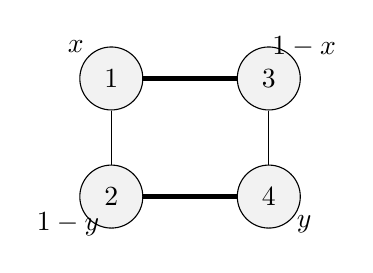
\begin{tikzpicture}[
                node/.style={circle, draw, fill=gray!10, minimum size=0.8cm},
                exchange/.style={line width=1.5pt},
                other/.style={line width=0.5pt}
            ]
            \node[node] (one) at (0, 1.5) {1};
            \node[node] (three) at (2, 1.5) {3};
            \node[node] (two) at (0, 0) {2};
            \node[node] (four) at (2, 0) {4};
            \draw[exchange] (one) -- (three);
            \draw[other] (one) -- (two);
            \draw[other] (three) -- (four);
            \draw[exchange] (two) -- (four);
            \node at (-0.45, 1.9) {$x$};
            \node at (2.45, 1.9) {$1-x$};
            \node at (-0.55, -0.35) {$1-y$};
            \node at (2.45, -0.35) {$y$};
        \end{tikzpicture}
        \caption{Network exchange with exchanging edges shown in bold.}
        \label{fig:hw7-four-node}
    \end{figure}
\end{problem}

\subsection{}
\begin{problem}
    If \(x=y=0.3\) in \cref{fig:hw7-four-node}, is the outcome stable? Is it balanced? Explain.
\end{problem}

\begin{solution}
    \begin{figure}[H]
        \centering
        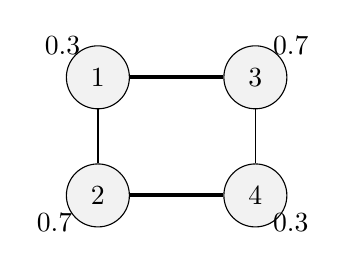
\begin{tikzpicture}[
                node/.style={circle, draw, fill=gray!10, minimum size=0.8cm},
                exchange/.style={line width=1.5pt},
                other/.style={line width=0.5pt}
            ]
            \node[node] (one) at (0, 1.5) {1};
            \node[node] (three) at (2, 1.5) {3};
            \node[node] (two) at (0, 0) {2};
            \node[node] (four) at (2, 0) {4};
            \draw[exchange] (one) -- (three);
            \draw[other] (one) -- (two);
            \draw[other] (three) -- (four);
            \draw[exchange] (two) -- (four);
            \node at (-0.45, 1.9) {$0.3$};
            \node at (2.45, 1.9) {$0.7$};
            \node at (-0.55, -0.35) {$0.7$};
            \node at (2.45, -0.35) {$0.3$};
        \end{tikzpicture}
    \end{figure}
    \begin{itemize}
        \item[$\checkmark$] Stable: all unused edges add to 1
        \item[$\checkmark$] Balanced: nodes are trading at values equal to their best outside option
    \end{itemize}
\end{solution}

\subsection{}
\begin{problem}
    If \(x=0.3\) and \(y=0.4\), is the outcome stable? Is it balanced? Explain.
\end{problem}
\begin{solution}
    \begin{figure}[H]
        \centering
        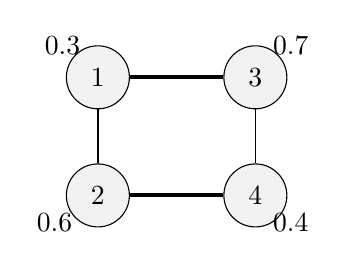
\begin{tikzpicture}[
                node/.style={circle, draw, fill=gray!10, minimum size=0.8cm},
                exchange/.style={line width=1.5pt},
                other/.style={line width=0.5pt}
            ]
            \node[node] (one) at (0, 1.5) {1};
            \node[node] (three) at (2, 1.5) {3};
            \node[node] (two) at (0, 0) {2};
            \node[node] (four) at (2, 0) {4};
            \draw[exchange] (one) -- (three);
            \draw[other] (one) -- (two);
            \draw[other] (three) -- (four);
            \draw[exchange] (two) -- (four);
            \node at (-0.45, 1.9) {$0.3$};
            \node at (2.45, 1.9) {$0.7$};
            \node at (-0.55, -0.35) {$0.6$};
            \node at (2.45, -0.35) {$0.4$};
        \end{tikzpicture}
    \end{figure}
    \begin{itemize}
        \item[$\times$] Unstable: Edge $(1,2)$ adds to 0.9, they would exchange to improve payoffs
        \item[$\times$] Unbalanced: unstable
    \end{itemize}
\end{solution}

\subsection{}
\begin{problem}
    Give an outcome of the network exchange in \cref{fig:hw7-four-node} that simultaneously satisfies the following two conditions: (i) the outcome is balanced; and (ii) adding one new non-exchanging edge to the network would make the outcome unbalanced. Explain why the outcome satisfies both conditions.

    \textit{Note: For parts c and d, you need to consider what would happen if you add a new non-exchanging edge between two of the nodes that are already in the network—without adding any new nodes.}
\end{problem}

\begin{solution}
    Add the edge between nodes 1 and 4:
    \begin{figure}[H]
        \centering
        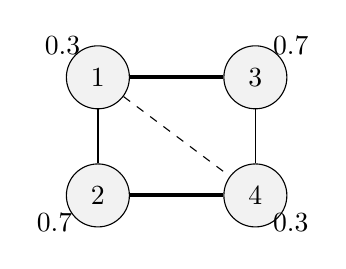
\begin{tikzpicture}[
                node/.style={circle, draw, fill=gray!10, minimum size=0.8cm},
                exchange/.style={line width=1.5pt},
                other/.style={line width=0.5pt}
            ]
            \node[node] (one) at (0, 1.5) {1};
            \node[node] (three) at (2, 1.5) {3};
            \node[node] (two) at (0, 0) {2};
            \node[node] (four) at (2, 0) {4};
            \draw[exchange] (one) -- (three);
            \draw[other] (one) -- (two);
            \draw[other] (three) -- (four);
            \draw[exchange] (two) -- (four);
            \draw[dashed] (one) -- (four);
            \node at (-0.45, 1.9) {0.3};
            \node at (2.45, 1.9) {0.7};
            \node at (-0.55, -0.35) {0.7};
            \node at (2.45, -0.35) {0.3};
        \end{tikzpicture}
    \end{figure}
    Nodes 1 and 4 each receive \(0.3\), so their payoffs on the new edge sum to \(0.6<1\), so it's unstable and unbalanced.
\end{solution}

\subsection{}
\begin{problem}
    Give an outcome of the network exchange in \cref{fig:hw7-four-node} that simultaneously satisfies the following two conditions: (i) the outcome is balanced; and (ii) there's no way to add a new non-exchanging edge to make it unbalanced. Explain why the outcome satisfies both conditions.

    An equivalent way of explaining the conditions in part d: (i) the outcome is balanced; and (ii) no matter what new non-exchanging edge you add to the network, the network remains balanced.
\end{problem}

\begin{solution}
    Use \(x=y=0.5\):

    \begin{figure}[H]
        \centering
        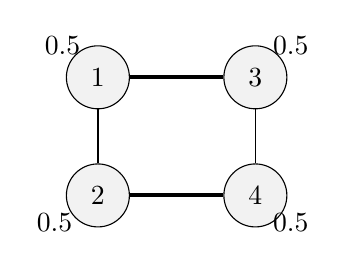
\begin{tikzpicture}[
                node/.style={circle, draw, fill=gray!10, minimum size=0.8cm},
                exchange/.style={line width=1.5pt},
                other/.style={line width=0.5pt}
            ]
            \node[node] (one) at (0, 1.5) {1};
            \node[node] (three) at (2, 1.5) {3};
            \node[node] (two) at (0, 0) {2};
            \node[node] (four) at (2, 0) {4};
            \draw[exchange] (one) -- (three);
            \draw[other] (one) -- (two);
            \draw[other] (three) -- (four);
            \draw[exchange] (two) -- (four);
            \node at (-0.45, 1.9) {0.5};
            \node at (2.45, 1.9) {0.5};
            \node at (-0.55, -0.35) {0.5};
            \node at (2.45, -0.35) {0.5};
        \end{tikzpicture}
    \end{figure}

    All nodes receive \(0.5\), and each unused edge gives both nodes an outside option of \(0.5\), so the outcome is balanced. On the diagonals, the payoffs sum to \(0.5+0.5=1\), so neither edge is unstable. The diagonals also give their nodes outside options of \(0.5\), keeping the existing exchanges balanced. Therefore, adding any new unused edge between existing nodes keeps the outcome balanced.
\end{solution}

\section{A Five-Participant Network}

\begin{problem}
    (20 Points) Consider a network exchange experiment with five participants, A, B, C, D, and E, connected as shown in \cref{fig:hw7-path}. Each edge represents a possible exchange relationship. In each round, a participant can exchange with at most one neighbor. Each exchange generates a total of \$10, which the two participants divide between themselves.

    \begin{figure}[H]
        \centering
        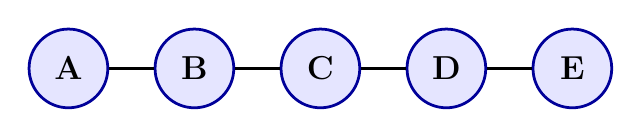
\begin{tikzpicture}[
                person/.style={circle, draw=blue!60!black, fill=blue!10, line width=1pt, minimum size=1cm, font=\large\bfseries}
            ]
            \foreach \name/\x in {A/0, B/1.6, C/3.2, D/4.8, E/6.4} {
                    \node[person] (\name) at (\x, 0) {\name};
                }
            \draw[line width=1pt] (A) -- (B) -- (C) -- (D) -- (E);
        \end{tikzpicture}
        \caption{Five-participant network.}
        \label{fig:hw7-path}
    \end{figure}
\end{problem}

\subsection{}
\begin{problem}
    Which participant or participants would you expect to receive the largest share of the money in this network? Briefly explain your reasoning. You do not need to calculate exact payoffs.
\end{problem}

\begin{solution}
    I would expect nodes B and D to receive the most money in this network because they have the most connections, and they would be able to exploit nodes A and E. I would not include C in the highest earning nodes because it cannot exploit any leaf node.
\end{solution}

\subsection{}
\begin{problem}
    Suppose that A exchanges with B and C exchanges with D, while E does not exchange. A receives \(a\), B receives \(10-a\), C receives \(x\), and D receives \(10-x\). Determine the best outside option for each of A, B, C, and D in terms of \(a\) and \(x\).
\end{problem}

\begin{solution}
    \begin{figure}[H]
        \centering
        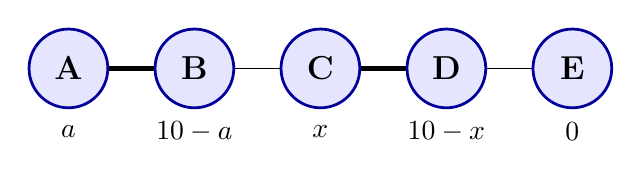
\begin{tikzpicture}[
                person/.style={circle, draw=blue!60!black, fill=blue!10, line width=1pt, minimum size=1cm, font=\large\bfseries},
                exchange/.style={line width=1.5pt},
                other/.style={line width=0.5pt}
            ]
            \foreach \name/\x in {A/0, B/1.6, C/3.2, D/4.8, E/6.4} {
                    \node[person] (\name) at (\x, 0) {\name};
                }
            \draw[exchange] (A) -- (B);
            \draw[other] (B) -- (C);
            \draw[exchange] (C) -- (D);
            \draw[other] (D) -- (E);
            \node at (0, -0.8) {$a$};
            \node at (1.6, -0.8) {$10-a$};
            \node at (3.2, -0.8) {$x$};
            \node at (4.8, -0.8) {$10-x$};
            \node at (6.4, -0.8) {$0$};
        \end{tikzpicture}
    \end{figure}

    Best outside options per node:
    \begin{itemize}
        \item[A:] 0, no outside option
        \item[B:] $10-x$ from C, since C must receive at least $x$
        \item[C:] $a$ from B, since B must receive at least $10-a$
        \item[D:] 10 from E, since E has no other exchange
    \end{itemize}
\end{solution}

\subsection{}
\begin{problem}
    Using the outside options from part b, determine the Nash bargaining solution for the exchange between A and B. Express the resulting payoffs for A and B in terms of \(x\).
\end{problem}

\begin{solution}
    A's and B's gains are $a$ and $(10-a)-(10-x)=x-a$. The Nash product is maximized when these gains are equal:
    \begin{equation}
        a=x-a
        \implies a=\frac{x}{2}
    \end{equation}

    Therefore, A receives $\boxed{\frac{x}{2}}$ and B receives $10-a=\boxed{10-\frac{x}{2}}$.
\end{solution}

\subsection{}
\begin{problem}
    Now suppose a sixth participant, F, joins the network and is connected only to C, as shown in \cref{fig:hw7-path-with-f}. Compared with the original network in part a, how would you expect the relative bargaining power of C and its neighbors to change? Explain your reasoning in terms of exchange opportunities and competition. You do not need to calculate exact payoffs.

    \begin{figure}[H]
        \centering
        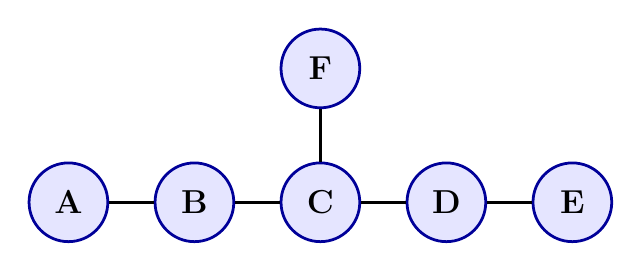
\begin{tikzpicture}[
                person/.style={circle, draw=blue!60!black, fill=blue!10, line width=1pt, minimum size=1cm, font=\large\bfseries}
            ]
            \foreach \name/\x in {A/0, B/1.6, C/3.2, D/4.8, E/6.4} {
                    \node[person] (\name) at (\x, 0) {\name};
                }
            \node[person] (F) at (3.2, 1.7) {F};
            \draw[line width=1pt] (A) -- (B) -- (C) -- (D) -- (E);
            \draw[line width=1pt] (F) -- (C);
        \end{tikzpicture}
        \caption{Five-participant network with F connected to C.}
        \label{fig:hw7-path-with-f}
    \end{figure}
\end{problem}

\begin{solution}
    I would expect C's bargaining power to increase because not only does it have more connections, but now one of those connections is a leaf node (F) which C can exploit. Previously, C was not the strongest because it couldn't exploit a leaf node while B and D could. Now, there are three nodes competing for its exchange while B and D only have two nodes each, so I would expect C to have more bargaining power than both B and D.
\end{solution}

\section{Stable and Balanced Outcomes}

\begin{problem}
    (25 Points) Consider a network exchange experiment on the network below. In the outcome of this exchange, A gets \$\(x\), where \(x\) can be any number between and including 0.5 and 1.

    \begin{figure}[H]
        \centering
        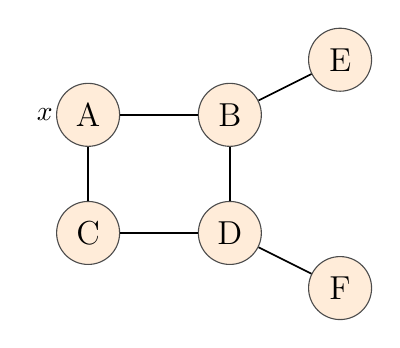
\begin{tikzpicture}[
                person/.style={circle, draw=black!70, fill=orange!15, minimum size=0.8cm, font=\large},
                edge/.style={line width=0.6pt}
            ]
            \node[person] (A) at (0, 1.5) {A};
            \node[person] (B) at (1.8, 1.5) {B};
            \node[person] (C) at (0, 0) {C};
            \node[person] (D) at (1.8, 0) {D};
            \node[person] (E) at (3.2, 2.2) {E};
            \node[person] (F) at (3.2, -0.7) {F};
            \draw[edge] (A) -- (B);
            \draw[edge] (A) -- (C);
            \draw[edge] (B) -- (D);
            \draw[edge] (C) -- (D);
            \draw[edge] (B) -- (E);
            \draw[edge] (D) -- (F);
            \node at (-0.55, 1.5) {$x$};
        \end{tikzpicture}
        \caption{Network exchange experiment for Problem 4.}
        \label{fig:hw7-stable-balanced}
    \end{figure}
\end{problem}

\subsection{}
\begin{problem}
    If the outcome is stable, which pairs of nodes must exchange with each other? Explain in 3--5 sentences.

    \textit{Hint: First, explain why, if B doesn't exchange with E, at least one edge will have an instability. Then, use the one-exchange rule to explain which other nodes have to exchange with each other if B-E is an exchanging edge.}
\end{problem}
\begin{solution}
    If B does not exchange with E, then E receives 0, so stability on B--E requires B to receive 1. Since A receives \(x>0\), B cannot exchange with A; B must exchange with D, leaving D and F with 0 and making D--F unstable. Therefore B exchanges with E. A must exchange with C to receive \(x>0\), and stability then requires D to exchange with F.
\end{solution}

\subsection{}
\begin{problem}
    Draw an example of a network exchange outcome that is stable but not balanced. Your example should specify which pairs of nodes negotiate an exchange and how much money each node receives. Show that your outcome is stable but not balanced.
\end{problem}

\begin{figure}[H]
    \centering
    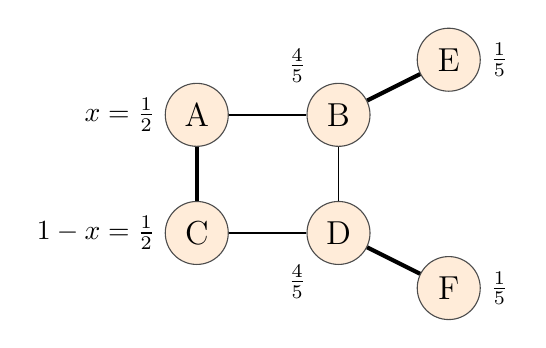
\begin{tikzpicture}[
            person/.style={circle, draw=black!70, fill=orange!15, minimum size=0.8cm, font=\large},
            edge/.style={line width=0.6pt},
            exchange/.style={line width=1.5pt}
        ]
        \node[person, label=left:{$x=\frac{1}{2}$}] (A) at (0, 1.5) {A};
        \node[person, label=above left:{$\frac{4}{5}$}] (B) at (1.8, 1.5) {B};
        \node[person, label=left:{$1-x=\frac{1}{2}$}] (C) at (0, 0) {C};
        \node[person, label=below left:{$\frac{4}{5}$}] (D) at (1.8, 0) {D};
        \node[person, label=right:{$\frac{1}{5}$}] (E) at (3.2, 2.2) {E};
        \node[person, label=right:{$\frac{1}{5}$}] (F) at (3.2, -0.7) {F};
        \draw[edge] (A) -- (B);
        \draw[exchange] (A) -- (C);
        \draw[edge] (B) -- (D);
        \draw[edge] (C) -- (D);
        \draw[exchange] (B) -- (E);
        \draw[exchange] (D) -- (F);
    \end{tikzpicture}
\end{figure}

\begin{solution}
    Unused edges:
    \[
        A+B=\frac{13}{10}\geq 1,\qquad B+D=\frac{8}{5}\geq 1,\qquad C+D=\frac{13}{10}\geq 1
        \implies \text{stable}.
    \]
    B's outside option is \(\max(1-A,1-D)=\frac12\), and E's is 0:
    \[
        B-\frac12=\frac{3}{10}\neq\frac15=E-0
        \implies \text{not balanced}.
    \]
\end{solution}

\subsection{}
\begin{problem}
    Draw an example of a network exchange outcome that is stable and balanced when \(x=0.5\). Your example should specify which pairs of nodes negotiated an exchange and how much money each node received. Show that your outcome is balanced.

    \textit{Hint: First figure out how much A and the node A is exchanging with get. Then solve the Nash bargaining equation for the edge B-E with the outside options you know. Finally solve the Nash bargaining equation for the third exchanging edge.}
\end{problem}

\begin{solution}
    \begin{figure}[H]
        \centering
        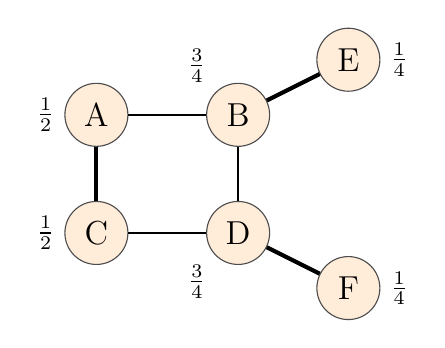
\begin{tikzpicture}[
                person/.style={circle, draw=black!70, fill=orange!15, minimum size=0.8cm, font=\large},
                edge/.style={line width=0.6pt},
                exchange/.style={line width=1.5pt}
            ]
            \node[person, label=left:{$\frac12$}] (A) at (0, 1.5) {A};
            \node[person, label=above left:{$\frac34$}] (B) at (1.8, 1.5) {B};
            \node[person, label=left:{$\frac12$}] (C) at (0, 0) {C};
            \node[person, label=below left:{$\frac34$}] (D) at (1.8, 0) {D};
            \node[person, label=right:{$\frac14$}] (E) at (3.2, 2.2) {E};
            \node[person, label=right:{$\frac14$}] (F) at (3.2, -0.7) {F};
            \draw[edge] (A) -- (B);
            \draw[exchange] (A) -- (C);
            \draw[edge] (B) -- (D);
            \draw[edge] (C) -- (D);
            \draw[exchange] (B) -- (E);
            \draw[exchange] (D) -- (F);
        \end{tikzpicture}
        \caption{Stable, balanced outcome for \(x=\frac12\); exchanges are bold.}
        \label{fig:hw7-balanced-half}
    \end{figure}

    B's outside option is \(\max(1-A,1-D)=\max(\frac12,\frac14)=\frac12\), and E's is 0. The Nash bargaining solution maximizes
    \[
        (B-\tfrac12)E \quad\text{where } B+E=1.
    \]
    Substituting \(E=1-B\) and maximize \((B-\frac12)(1-B)\), which is largest at \(B=\frac34\), so \(E=\frac14\). The same solution is for D and F.

    The unused-edge sums are \(\frac54,\frac32,\frac54\), so the outcome is stable. The outside options for \(A,B,C,D,E,F\) are \((\frac14,\frac12,\frac14,\frac12,0,0)\). Each participant gains \(\frac14\) over their outside option, so the outcome is balanced.
\end{solution}

\subsection{}
\begin{problem}
    Next, we'll walk you through some steps to specify all possible network exchange outcomes that are stable and balanced. We know that A gets \(x\geq 0.5\) from their exchange. In the next 4 steps, we'll see how we can figure out what the rest of the nodes get in terms of \(x\). This allows us to express all possible outcomes since for any value of \(x\):
    \begin{enumerate}[label=\roman*.]
        \item Who is A's exchanging partner, and how much do they get in terms of \(x\)?
        \item Show that, in a stable, balanced outcome, D gets a value of \(x\) or more.
        \item In a stable, balanced outcome, how much do B and E get in terms of \(x\)? Show your work, including how you calculate each node's outside options and apply the Nash bargaining solution.
        \item There's one final exchanging pair whose split we haven't yet calculated. In a stable, balanced outcome, how much does each of them get in terms of \(x\)? Show your work, including how you calculate each node's outside options and apply the Nash bargaining solution.
    \end{enumerate}
\end{problem}

\begin{solution}
    Write each participant's letter for their payoff.
    \begin{enumerate}[label=\roman*.]
        \item A exchanges with C, so \(C=1-x\).
        \item Stability on C--D gives \(C+D\geq 1\implies D\geq x\).
        \item For B--E, the outside options are \(\max(1-x,1-D)=1-x\) and 0 so
              \[
                  B-(1-x)=E,\qquad B+E=1
                  \implies B=1-\frac{x}{2},\quad E=\frac{x}{2}.
              \]
        \item For D--F, the outside options are \(\max(1-C,1-B)=x\) and 0 so
              \[
                  D-x=F,\qquad D+F=1
                  \implies D=\frac{1+x}{2},\quad F=\frac{1-x}{2}.
              \]
    \end{enumerate}
\end{solution}

\subsection{}
\begin{problem}
    Check your work: If you plug in \(x=0.5\) to your answers from part d, do you get your answers from part c?
\end{problem}

\begin{solution}
    \begin{align*}
        A & = x = \boxed{\frac12}          \\
        B & =1-\frac{x}{2}=\boxed{\frac34} \\
        C & = 1 - x = \boxed{\frac12}      \\
        D & =\frac{1+x}{2}=\boxed{\frac34} \\
        E & =\frac{x}{2}=\boxed{\frac14}   \\
        F & =\frac{1-x}{2}=\boxed{\frac14}
    \end{align*}

    This is the same result as \cref{fig:hw7-balanced-half}.
\end{solution}

\subsection{}
\begin{problem}
    Notice that node D never gets less than node B in the outcome, suggesting that D has more power than B. What about D's position in the network makes this the case? Offer a 1--3 sentence intuitive explanation.
\end{problem}

\begin{solution}
    B and D have symmetric positions, so swapping B with D, A with C, and E with F leaves the network exactly the same. The only stable, balanced outcome has \(B=D=\frac34\), so they have the same bargaining power.
\end{solution}

\section{HITS}

\begin{problem}
    Consider the webpage network below. Pages A--F are potential hubs and pages W--Z are potential authorities. Start with every hub score and every authority score equal to 1.
    \begin{figure}[H]
        \centering
        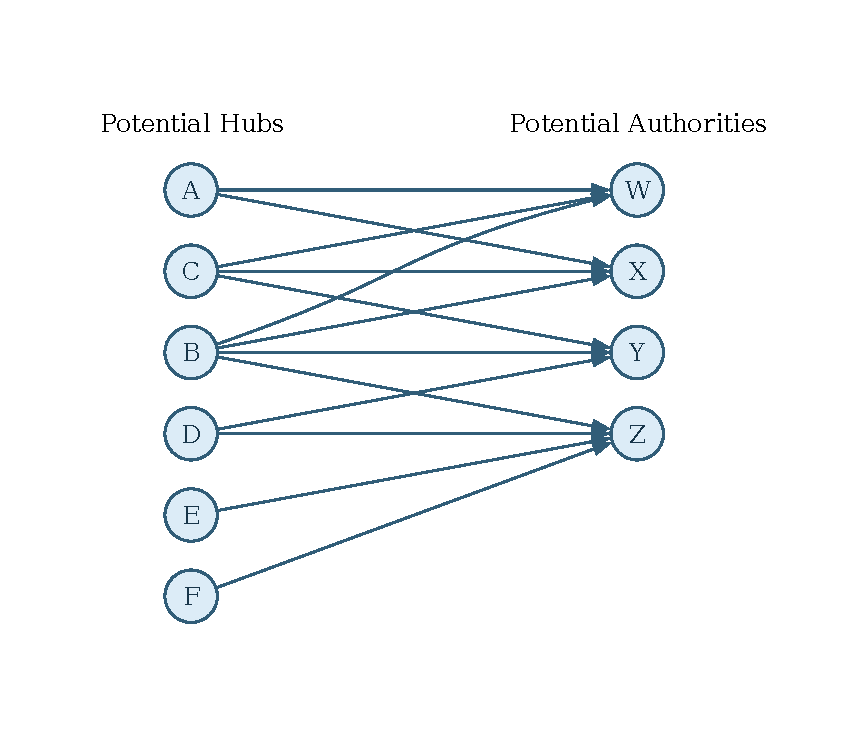
\includegraphics[height=0.5\textwidth]{figures/hits-network.pdf}
        \caption{Webpage network for the HITS updates.}
        \label{fig:hw7-hits}
    \end{figure}
\end{problem}


\subsection{}
\begin{problem}
    Run two full HITS updates on the network in \cref{fig:hw7-hits}. Fill in the table with the authority scores for W--Z and the hub scores for A--F after each update. Then report the normalized scores.

\end{problem}

\begin{table}[h]
    \caption{Two HITS updates on the original network.}
    \centering
    \begin{tabular}{ccccccccccc}
        \toprule
        Scores     & W      & X      & Y      & Z      & A      & B      & C      & D      & E      & F      \\
        \midrule
        Update \#1 & 3      & 3      & 3      & 4      & 6      & 13     & 9      & 7      & 4      & 4      \\
        Update \#2 & 28     & 28     & 29     & 28     & 56     & 113    & 85     & 57     & 28     & 28     \\
        \midrule
        Normalized & 0.4955 & 0.4955 & 0.5132 & 0.4955 & 0.3350 & 0.6759 & 0.5085 & 0.3410 & 0.1675 & 0.1675 \\
        \bottomrule
    \end{tabular}
\end{table}

\subsection{}
\begin{problem}
    Which page has the highest normalized authority score, and which page has the highest normalized hub score after two updates? Briefly explain why each page scores highly using the HITS intuition.
\end{problem}

\begin{solution}
    Page \textbf{Y} has the highest authority score ($29 = 0.5132$) and \textbf{B} has the highest hub score ($113 = 0.6759$). For Y, it's not just because Y has many hubs pointing to it because it has 3 like most other authorities. What gives Y the higher score is the \textbf{quality of the hubs that point to it}, which have high quality because they point to many authorities. Similarly for B, it \textbf{points at 4 authorities}, which is more than all other hubs. Also, the authorities that it points at are all good quality (mostly the same).
\end{solution}

\subsection{}
\begin{problem}
    Page A is allowed to add exactly one new outgoing link while keeping its existing links to W and X. It can add either \(A\to Y\) or \(A\to Z\). Starting again with all hub and authority scores equal to 1, which option gives A the larger normalized hub score after two full HITS updates? Show enough calculation to justify your answer.
\end{problem}

\begin{solution}

    \begin{table}[h]
        \caption{\(A\to Y\)}
        \centering
        \begin{tabular}{ccccccccccc}
            \toprule
            Scores     & W & X & Y & Z & A      & B   & C   & D  & E  & F  \\
            \midrule
            Update \#1 & 3 & 3 & 4 & 4 & 10     & 14  & 10  & 8  & 4  & 4  \\
            Update \#2 &   &   &   &   & 110    & 140 & 110 & 72 & 30 & 30 \\
            \midrule
            Normalized &   &   &   &   & 0.4881 &     &     &    &    &    \\
            \bottomrule
        \end{tabular}
    \end{table}

    \begin{table}[h]
        \caption{\(A\to Z\)}
        \centering
        \begin{tabular}{ccccccccccc}
            \toprule
            Scores     & W & X & Y & Z & A      & B   & C  & D  & E  & F  \\
            \midrule
            Update \#1 & 3 & 3 & 3 & 5 & 11     & 14  & 9  & 8  & 5  & 5  \\
            Update \#2 &   &   &   &   & 111    & 142 & 99 & 74 & 43 & 43 \\
            \midrule
            Normalized &   &   &   &   & 0.4893 &     &    &    &    &    \\
            \bottomrule
        \end{tabular}
    \end{table}

    Adding \(A\to Z\) gives A the slightly larger normalized hub score of 0.4893 rather than 0.4881 from $A \to Y$.
\end{solution}

\end{document}